\documentclass[conference]{IEEEtran}
\IEEEoverridecommandlockouts
\usepackage{cite}
\usepackage{amsmath,amssymb,amsfonts}
\usepackage{graphicx}
\usepackage{textcomp}
\usepackage{xcolor}
\usepackage{booktabs}
\usepackage{tabularx}
\usepackage{array}
\usepackage{float}
\usepackage{url}
\usepackage{caption}
\captionsetup{font=small,labelfont=bf}

\Urlmuskip=0mu plus 2mu\relax
\def\UrlBreaks{\do\/\do-\do\_\do\.\do\?\do\=\do\&}
\emergencystretch=2em

\graphicspath{{results/presentation/}{results/}}
\newcolumntype{Y}{>{\raggedright\arraybackslash}X}
\newcommand{\pjbit}{pJ/bit}
\newcommand{\tbps}{Tb/s}
\newcommand{\figref}[1]{Fig.~\ref{#1}}
\newcommand{\tabref}[1]{Table~\ref{#1}}
\newcommand{\secref}[1]{Sec.~\ref{#1}}

\def\BibTeX{{\rm B\kern-.05em{\sc i\kern-.025em b}\kern-.08em
    T\kern-.1667em\lower.7ex\hbox{E}\kern-.125emX}}

\begin{document}

\title{Photonic Interconnects for TPU LLM Workloads}

\author{
\IEEEauthorblockN{Pranav Sitaraman}
\IEEEauthorblockA{\textit{MIT 6.5930} \\ sitaraman.pranav@gmail.com}
\and
\IEEEauthorblockN{Simone Surdi}
\IEEEauthorblockA{\textit{MIT 6.5930} \\ simonesurdi@gmail.com}
}

\maketitle

\section{Introduction}
Frontier large language models are trained and served on TPU pods
whose performance is bounded less by raw matrix-multiply throughput
than by the cost of moving activations, KV-cache state, expert
tokens, gradients, optimizer state, and shared weights between
thousands of accelerators. Google's open-weight Gemma~4 family and
its proprietary Gemini~3 family run on TPU v5p and the 9216-chip
Ironwood/TPU7x pod, both of which are organised around high-radix
inter-chip interconnect because data movement is the limiter at
scale~\cite{tpuv5p,tpu7x,ironwood-blog}. Co-packaged photonic
interconnect---of which Lightmatter's Passage family is a public
reference point---offers lower per-bit energy and, more
interestingly, distance-insensitive transmission and hardware
multicast. We ask whether photonics is a constant-factor link
substitution or whether it changes \emph{how a TPU pod should be
mapped and scheduled}.

The danger in answering this question naively is that ``mapping''
already has a precise meaning: it is the joint choice of
partitioning, dataflow (stationarity), tile sizing, and storage
residency for a given accelerator and
workload~\cite{lec05-mapping,lec06-partitioning}. If the mapper is
not given a chance to react to the new technology, any improvement
measured is tautological. Conversely, if a per-chip mapping does
not move under a new fabric, the right conclusion is that the
benefit lives somewhere else, not that there is no benefit.

\textbf{Three insights follow from the study.}
First, the per-chip mapping is invariant under photonics: across
all twenty-four (workload, technology, communication-scenario)
combinations on a 64-chip cube, the optimal partitioning,
dataflow, and tile signature is unchanged. The local GEMM is
compute- and SRAM-bound, and photonics does not move those costs.
Second, the cluster-level schedule \emph{does} move: five of
sixteen workload--scenario pairs flip their preferred
communication pattern, and a strong 3.5~\tbps{}, 6~\pjbit{}
chiplet baseline---chosen specifically to defeat the bandwidth
hypothesis---is still beaten by the optical-circuit-switched M1000
by 99.85\% on shared-state multicast. Hardware multicast, which
collapses an $N$-way unicast fanout to a single logical broadcast,
is the decisive property. Third, photonics is not a uniform
multiplier: on the 9216-chip Ironwood pod, the Gemma~4 26B
sparse-MoE proxy reaches 42.43$\times$ inference latency speedup,
while training reaches only 3.37$\times$ because once collectives
shrink it becomes compute-dominated.

\section{Related Work}
\label{sec:related}

\textbf{Optimal accelerator mapping.}
The course formalism treats a mapping as the joint choice of
partitioning, dataflow, tile sizing, and storage
residency~\cite{lec05-mapping,lec06-partitioning}. The Turbo-Charged
Mapper (TCM) sharpens this view by adding dataplacement as a
first-class axis and shows that heuristic mappers can make
hardware comparisons misleading because they may miss the optimal
point in a mapspace that, for a GPT-3 attention example, contains
16 dataplacements, roughly $10^{15}$ dataflows, and $10^{22}$
tile-shape choices~\cite{tcm}. We follow the same discipline: a
hardware benefit only counts if the mapper had the chance to
react, and a non-moving mapping is reported rather than
concealed.

\textbf{Photonic accelerator modelling.}
CiMLoop for Photonics extends the Timeloop/Accelergy stack with
photonic component models for the full electrical, analog,
optical, and digital pipeline of a single
accelerator~\cite{ciml-photonics}. The present work is
complementary at the cluster scale: each chip's compute and memory
hierarchy is held fixed, and the question is how the inter-chip
fabric reshapes the schedule above the mapper.

\textbf{Lightmatter Passage and Google TPU pods.}
EVK100 reports 3.2~\tbps{} per fiber and energy efficiency in the
1.9--3.2~\pjbit{} range~\cite{lightmatter-evk100,
lightmatter-passage}. The M1000 evaluation kit reports
114.6~\tbps{} aggregate bidirectional bandwidth, 2.3~\pjbit{}
including laser power, and a built-in solid-state optical circuit
switch~\cite{lightmatter-m1000}. The L200 family and the OCP
co-packaged optics reference initiative provide additional public
anchors for switched optical fabrics~\cite{lightmatter-l200,
lightmatter-ocp,lightmatter-tco}. Public Cloud TPU documentation
specifies TPU7x at 4614~FP8 TFLOP/s per chip, 192~GiB HBM,
7.4~TB/s HBM bandwidth, 1200~GB/s bidirectional ICI per chip, with
the 9216-chip pod composed of $4{\times}4{\times}4$ cubes
\cite{tpu7x,ironwood-blog,hotchips-ironwood}.

\textbf{Compiler-visible distributed schedules.}
XLA/GSPMD and PyTorch/XLA SPMD describe how compilers shard
tensors and lower collectives~\cite{xla-spmd}; this is the layer
above the per-chip mapper at which photonics changes the design
space. We do not implement an XLA pass. We model four schedule
families that an XLA-style compiler would expose---sharded
collectives, remote pooled-HBM streaming, replicated cache, and
photonic multicast cache fill---and ask which is preferred when
the interconnect changes. Course material on advanced
technologies frames photonics in this same
direction~\cite{lec11-advtech}.

\section{Approach}
\label{sec:approach}

\subsection{Modelling stack: four layers, two of which can move}
The pipeline has four explicit layers; results are reported
separately at each. The first is the \emph{workload}, expressed as
the matrix-multiply einsum $O_{m,n}=\sum_k A_{m,k} W_{k,n}$ with
rank sizes drawn from each LLM stage. The second is the
\emph{architecture}: a logical cluster-scale memory level above
per-chip HBM, a node-array fanout that captures how many chips a
tile is spread across, an on-chip unified buffer, the
processing-element fanout with input and output reuse, a weight
register, and the MAC. The third is the \emph{mapping}, which is
what an architecture-aware mapper produces given a workload and
architecture: a sequence of storage, spatial, temporal, and
compute directives with concrete tile shapes. This is the course
definition of mapping~\cite{lec05-mapping}. The fourth is the
\emph{distributed schedule} that lives \emph{above} the mapper:
which tensor a compiler keeps in the cluster-wide pool versus
per-chip HBM, and which named XLA-style policy (sharded
collective, remote streaming, replicated cache, or photonic
multicast cache fill) the compiler selects. ``Dataflow'' here
means intra-PE stationarity; ``distributed dataflow strategy''
means the layer-4 inter-chip movement pattern. Both are reported
because photonics changes one and leaves the other alone.

\subsection{Physics: distance-parametrised link energy}
\label{sec:physics}
A flat per-bit constant hides the central asymmetry between
electrical and photonic links. Electrical links pay a small
conversion overhead at the SerDes and a transmission cost that
grows with distance because resistance and dielectric loss
accumulate along a copper trace. Photonic links pay a large
conversion overhead at the modulators, detectors, and laser, but
the actual transmission---photons moving through fibre or
waveguide---is essentially distance-free. Bit energy over $h$
hops of average physical link length $\ell(N)$ is therefore
\begin{equation}
E_{\text{bit}}(N) = e_c + h\,\ell(N)\,e_{tx/\text{mm}},
\label{eq:ebit}
\end{equation}
where $e_c$ is conversion energy and $e_{tx/\text{mm}}$ is per-mm
transmission energy. Each technology is calibrated so that its
published reference value is recovered at a representative
distance: the high-speed electrical points contribute most of
their energy in the transmission term, and each Lightmatter
Passage point is dominated by the conversion term with
$e_{tx/\text{mm}}$ on the order of $5{\times}10^{-5}$~\pjbit{}
per millimetre. Total network cost combines bandwidth, hop,
propagation, and switching:
\begin{equation}
T_{\text{net}}(N) = \frac{B}{BW_\ell/C(N)} + h\,t_r
                  + h\,\ell(N)\,t_p + t_s ,
\end{equation}
with contention $C(N)$ equal to $\sqrt{N}$ for a 2-D mesh,
$\sqrt[3]{N}$ for a 3-D torus, and one for a switched fabric.
Multicast is the other key knob: a non-multicast technology pays
the unicast volume $N$ times for an $N$-way fanout, while a
multicast-capable photonic technology pays the unique payload
once. Optical-circuit-switching variants pay an explicit
reconfiguration term $t_s$; the optical-packet-switching
sensitivity model pays an additional per-packet term but avoids
$t_s$.

\subsection{Iterative feedback into the mapper}
The mapper does not natively model the inter-chip network. The
cluster pool is exposed as a logical memory level whose energy
and latency can be updated. After each mapper run the
cluster-level read and write traffic is read out, priced by
Eq.~\ref{eq:ebit}, and folded back into the energy and latency of
that level. The mapper is then re-run. The loop converges to a
fixed point in three iterations or fewer in every case
evaluated, after which both the energy and the mapping signature
are stable.

\subsection{End-to-end stage model}
For full-superpod inference and training each LLM
stage---prefill, decode KV attention, weight or expert refill,
MoE dispatch and combine, training forward and backward, gradient
synchronization, and optimizer state---decomposes into compute,
HBM, and network terms with an explicit overlap factor:
\begin{equation}
T_{\text{stage}} = \max(T_c, T_{\text{HBM}})
                 + (1-\alpha)\,T_{\text{net}} .
\end{equation}
Compute and HBM terms come from per-chip throughput and memory
bandwidth, the network term from the topology cost above, and
$\alpha\!\in\![0,1]$ models how much of the network transfer hides
behind compute. This is an analytical critical-path model rather
than a cycle-accurate simulator; it does not capture packet-level
queueing or optical-switch reconfiguration timing.

\section{Experiment Setup}
\label{sec:setup}

\textbf{Held fixed.}
Compute, register, on-chip buffer, per-chip HBM capacity, and
HBM energy and latency are identical across all comparisons.
Only interconnect technology, topology, and distributed schedule
vary.

\begin{table}[t]
\centering
\caption{Modelled interconnect technologies. Bandwidth is one-way
per link; energy is the public reference value at a representative
distance.}
\label{tab:tech}
\scriptsize
\setlength{\tabcolsep}{2.5pt}
\begin{tabular}{lrrcl}
\toprule
Technology         & BW          & Energy        & MC  & Mode \\
\midrule
Electrical 800G    & 0.8~\tbps   & 10.0~\pjbit   & --- & packet \\
Advanced chiplet   & 3.5~\tbps   & 6.0~\pjbit    & --- & packet \\
Lightmatter EVK50  & 0.8~\tbps   & 4.6~\pjbit    & yes & circuit \\
Lightmatter EVK100 & 3.2~\tbps   & 1.9~\pjbit    & yes & circuit \\
Lightmatter L200   & 16~\tbps    & 4.5~\pjbit    & yes & circuit \\
Lightmatter L200X  & 32~\tbps    & 4.8~\pjbit    & yes & circuit \\
Lightmatter M1000  & 57.3~\tbps  & 2.3~\pjbit    & yes & circuit \\
M1000 OPS sense    & 57.3~\tbps  & 2.9~\pjbit    & yes & packet \\
\bottomrule
\end{tabular}
\end{table}

\textbf{Baselines.}
The cluster experiment uses a 16-node electrical $4{\times}4$
mesh. The cube experiment uses the 64-chip $4{\times}4{\times}4$
TPU v5p-class electrical torus. The superpod baseline is an
Ironwood electrical torus with 9216 chips at the public per-chip
Ironwood specifications. The advanced chiplet baseline is included
so that any photonic gain reported cannot be explained by raw
bandwidth alone.

\textbf{Workloads.}
Six GEMM proxies for LLM stages drive the per-chip mapper study:
decode MLP, KV attention, prefill projection, long-context
prefill, MoE expert dispatch, and training weight gradient. The
end-to-end superpod study uses public Gemma~4 anchors---the 26B
sparse-MoE point and the 31B dense point with long-context
support---together with two Gemini-class stress proxies: a
Pro-class sparse-MoE workload at 4.7T total / 600B active
parameters and a Deep Think-class long-context workload at 4.7T /
750B / 131K context. Gemma~4 sizes are public; the Gemini stress
workloads are labelled as proxies because parameter counts are
not.

\textbf{Reproducibility.}
A single command rebuilds every artifact in the paper inside the
course's container image, including the regression suite that
asserts technology constants, the long-distance crossover, the
multicast-volume semantics, and the inference--training
asymmetry.

\textbf{Limitations.}
Optical multicast is modelled as one logical broadcast (an
optimistic, explicit assumption); the analytical stage model is
not cycle-accurate; the optical-packet-switching point is a
sensitivity what-if, not a Lightmatter product claim; Gemini
parameter counts are not public, so proxy stress workloads are
labelled as such.

\section{Results and Discussion}
\label{sec:results}

The results follow one tight chain: the physical asymmetry between
electrical and photonic links sets up the topology argument, the
topology argument sets up the layered mapping/schedule split, the
layered split sets up the scaling argument, and the scaling
argument sets up the end-to-end superpod story. Each subsection
takes the next step.

\subsection{Distance is where the crossover lives}
\label{sec:r-distance}

\figref{fig:distance} sweeps modelled active-chip count from cube
to pod scale and reports the effective \pjbit{} that one bit pays
at the average path distance in each topology. The electrical and
chiplet tori rise roughly an order of magnitude across the sweep
because their per-mm transmission term grows with the average
physical path. The two M1000 points (circuit and packet
switching) and the EVK100 photonic torus stay flat, because
their conversion terms dominate and their per-mm contribution is
negligible. Below roughly ten millimetres the electrical link
wins on raw \pjbit{}; near pod-scale path lengths it is two
orders of magnitude more expensive per bit. This crossover is the
physical reason photonic interconnect cannot be evaluated as a
flat constant.

\begin{figure}[t]
\centering
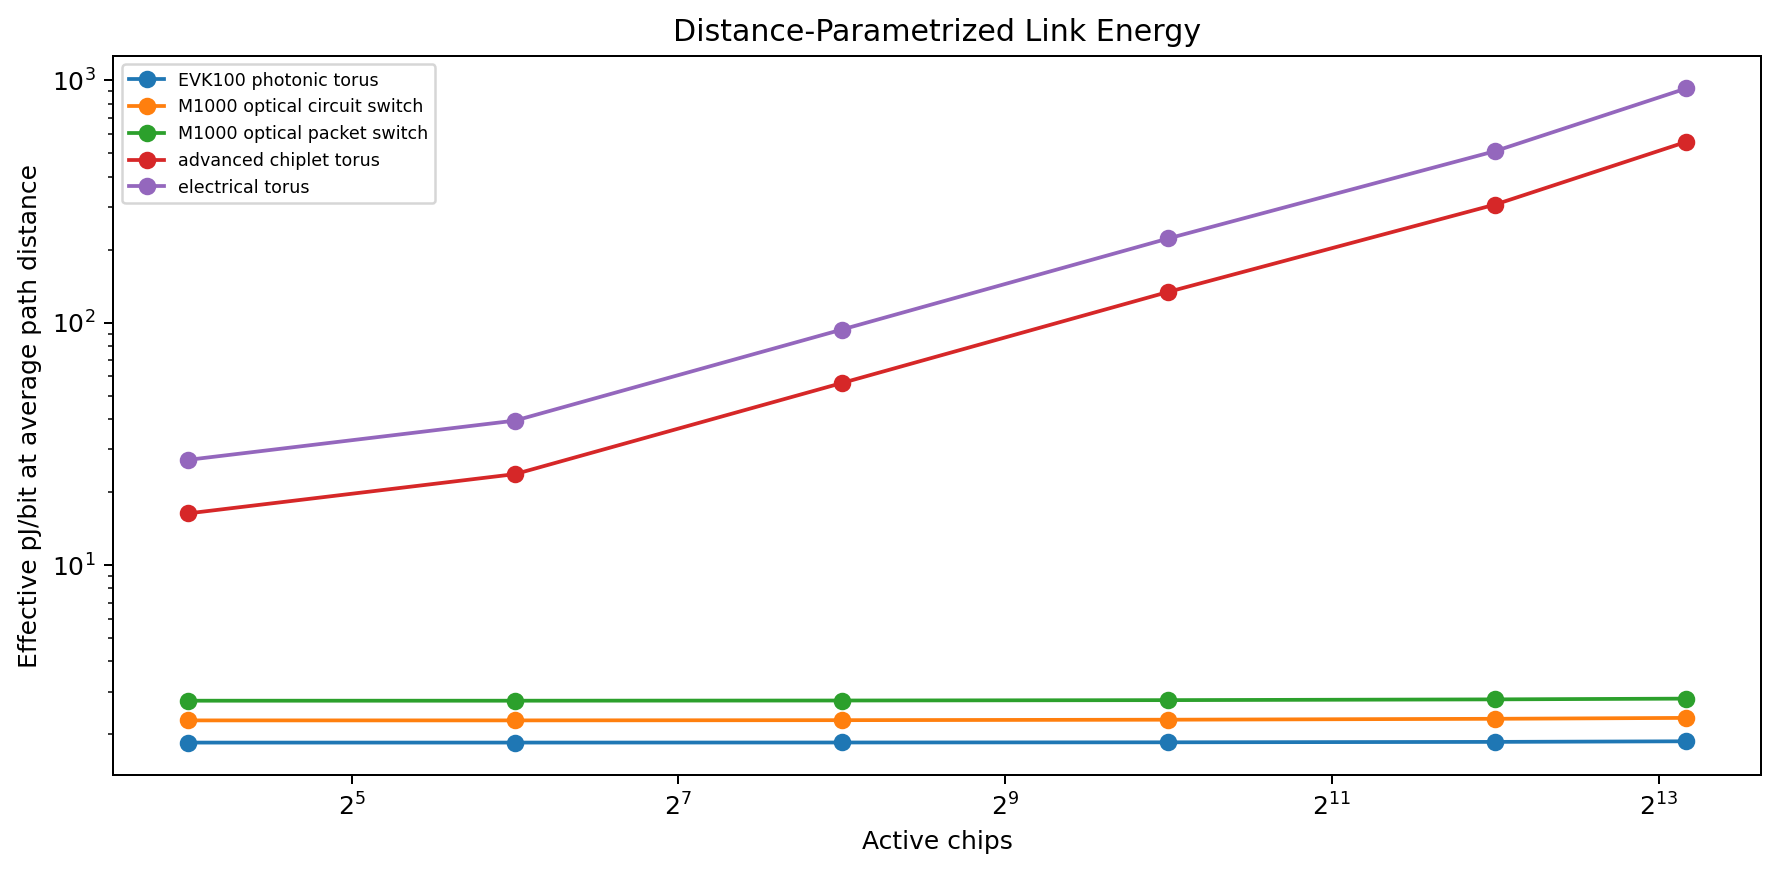
\includegraphics[width=0.97\linewidth]{10_distance_physics.png}
\caption{Effective \pjbit{} at the average path distance. The
electrical and chiplet tori rise nearly linearly with cluster
size; the photonic switched fabrics stay flat.}
\label{fig:distance}
\end{figure}

\subsection{Multicast, not bandwidth, is decisive}
\label{sec:r-multicast}

\figref{fig:tpu} shows AccelForge-mapped energy reduction on the
64-chip cube relative to the TPU v5p-class electrical torus,
broken down by communication scenario. On node-to-node activation
exchange, where the torus pays only one short hop, photonic gains
are modest. On shared-DRAM multicast, where the workload
broadcasts the same payload to many chips, the gain jumps to
about 99.93\% energy reduction for the EVK100 photonic torus and
99.91\% for the M1000 switched fabric.

The chiplet test in \figref{fig:chiplet} isolates the multicast
property from raw bandwidth. The 3.5~\tbps{}, 6~\pjbit{} chiplet
baseline closes most of the bandwidth gap on activation exchange
and remote-weight refill (87--92\% reduction), but on shared-state
multicast both EVK100 and M1000 still beat it by 99.85\%. The
reason is structural: $N$ unicasts collapse to one logical
broadcast, and the contention floor disappears on a switched
fabric. Multicast is the architectural property that matters,
not raw bandwidth.

\begin{figure}[t]
\centering
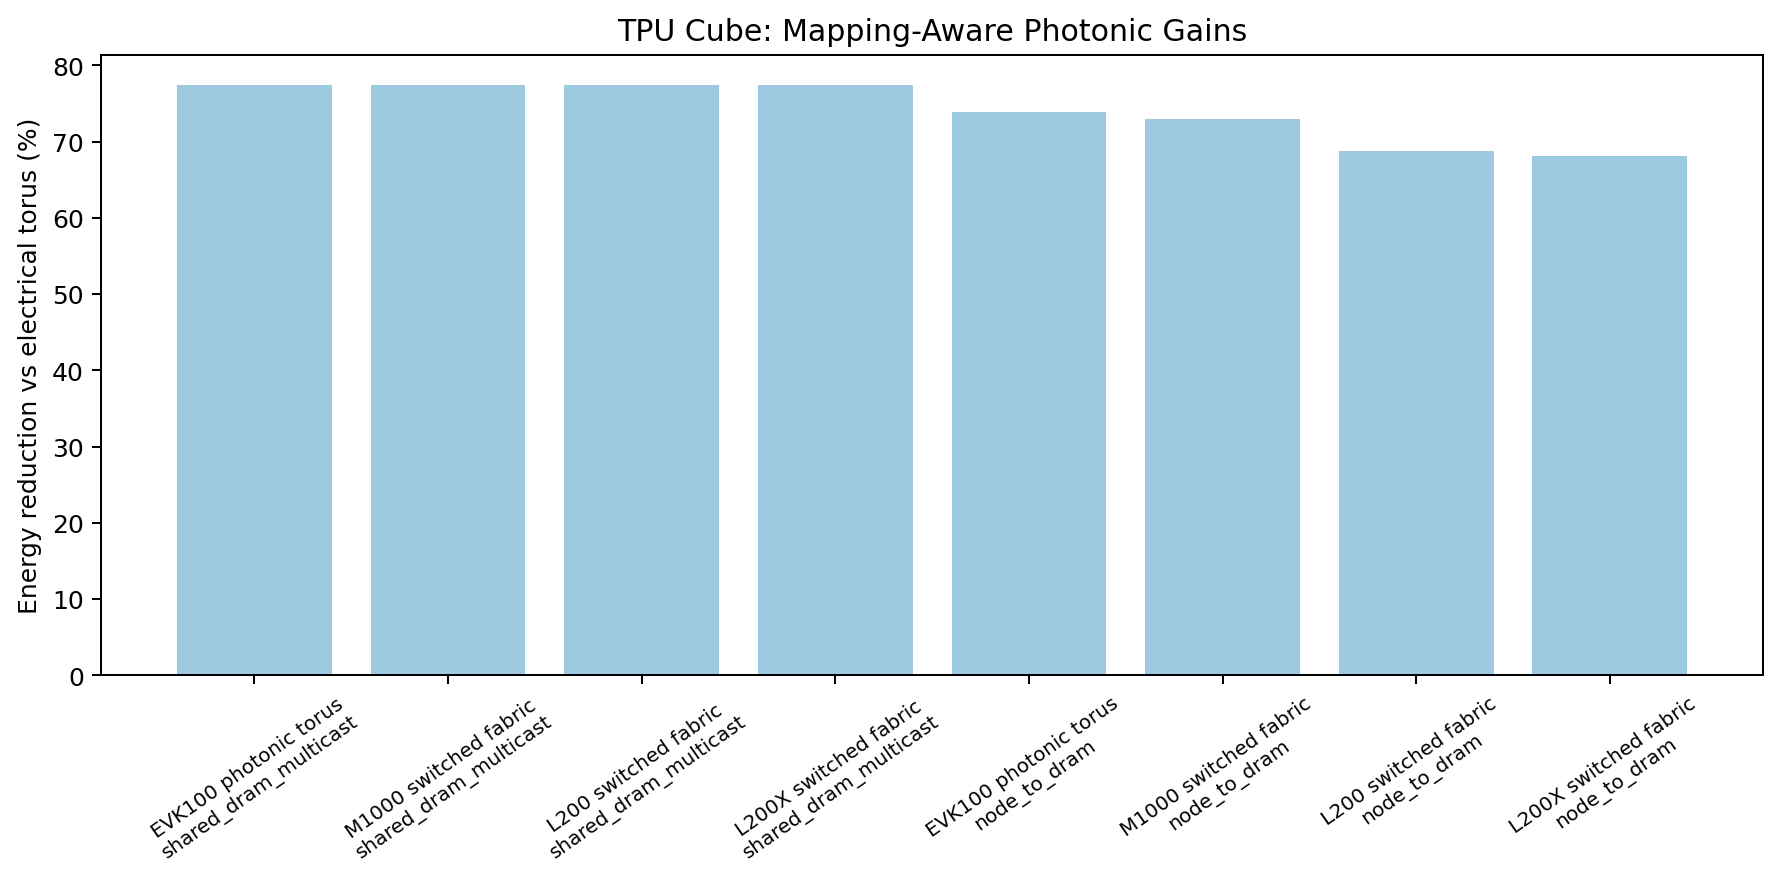
\includegraphics[width=0.97\linewidth]{02_tpu_mapping_reductions.png}
\caption{TPU-cube energy reduction relative to the electrical
torus under the same per-chip mapper. Multicast bars (left) cluster
near 77\%; node-to-DRAM bars (right) are smaller and depend more
on raw bandwidth.}
\label{fig:tpu}
\end{figure}

\begin{figure}[t]
\centering
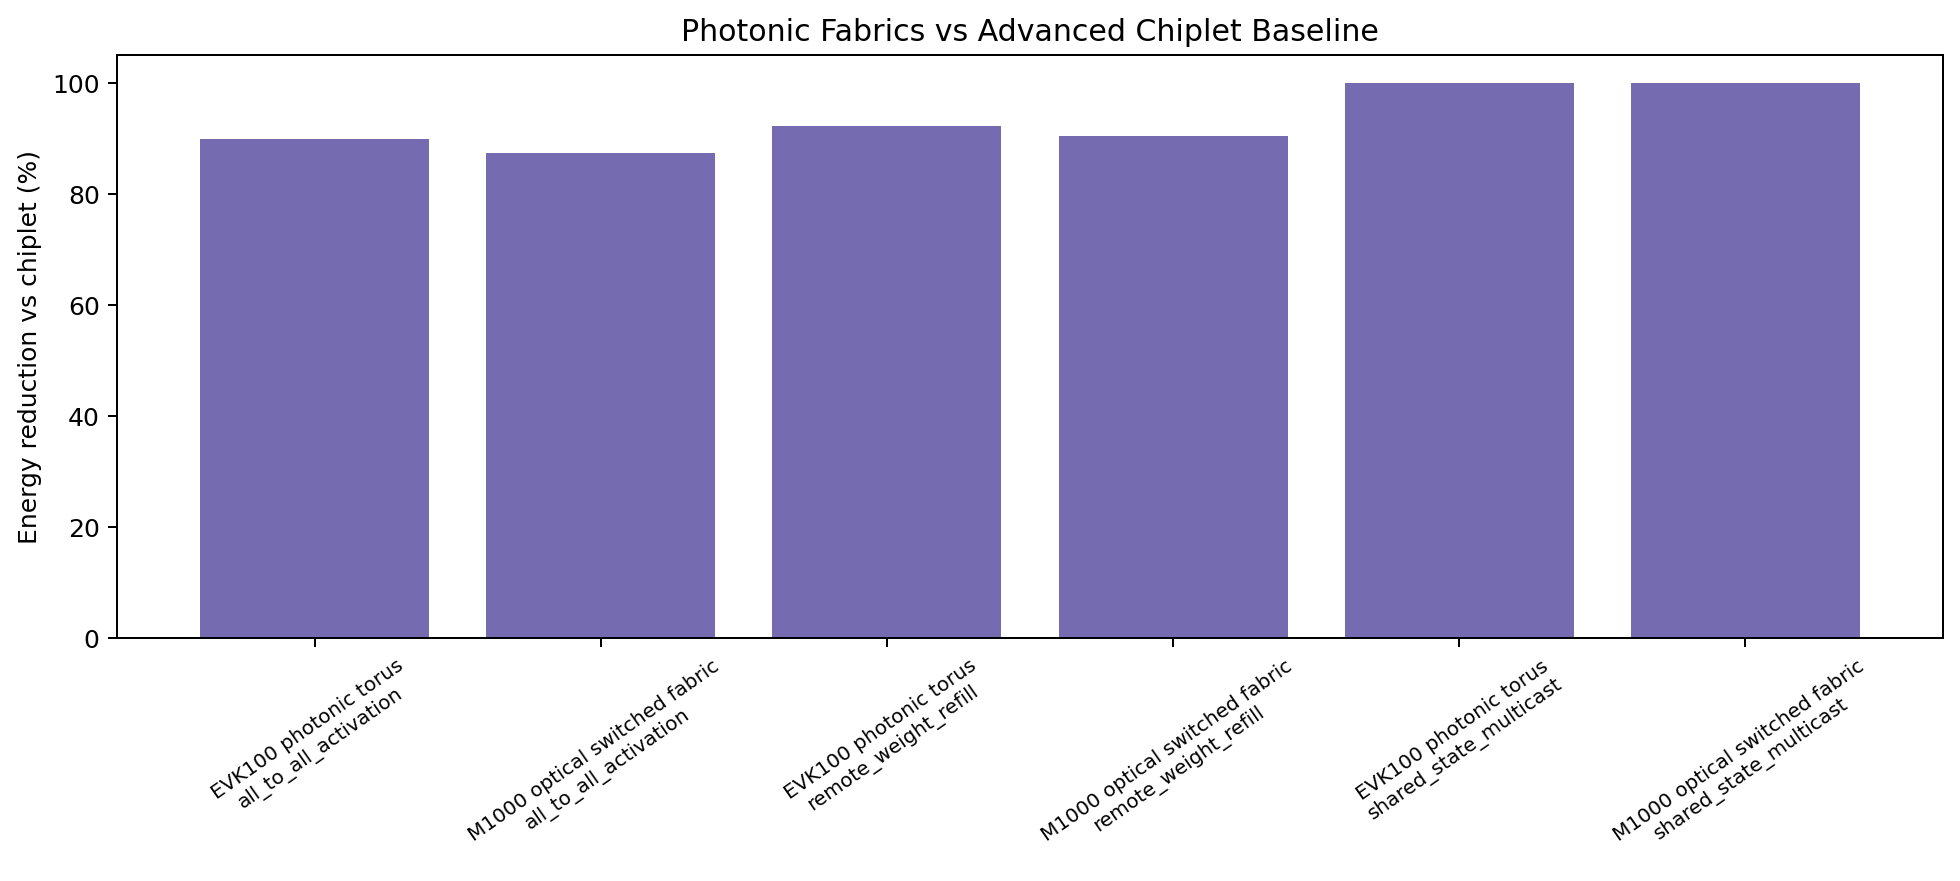
\includegraphics[width=0.97\linewidth]{06_chiplet_baseline.png}
\caption{Photonic fabrics versus the strong 3.5~\tbps{},
6~\pjbit{} chiplet baseline. The bandwidth hypothesis is defeated
on shared-state multicast: M1000 still beats the chiplet by
99.85\%.}
\label{fig:chiplet}
\end{figure}

\subsection{The mapping is invariant; the schedule moves}
\label{sec:r-mapping}

The most interesting finding is the cleanly two-layered behaviour
of photonics. Across the twenty-four (workload, technology,
communication-scenario) combinations on the cube, the mapper
converges to the same spatial-fanout, residency, and
action-count signature for every photonic and chiplet variant:
zero of twenty-four signatures change. The per-chip GEMM is
dominated by local compute and SRAM-/HBM-level reuse, neither of
which photonics moves.

The benefit lives one layer higher. Five of sixteen
workload--scenario pairs in the distributed-mapping study flip
their preferred communication pattern from node-to-node exchange
to shared-DRAM multicast under a photonic technology, because the
multicast volume cost has collapsed. \figref{fig:compiler}
reports the energy gain of the best XLA-style schedule per
(workload, technology) cell. Remote pooled-HBM streaming on
EVK100 removes 73.86\% of the compute energy on KV attention, and
photonic multicast cache fill becomes the dominant choice for
shared-state KV and expert refill whenever multicast is
available. The chiplet baseline cannot make any of these
schedule changes because it lacks multicast.

\begin{figure}[t]
\centering
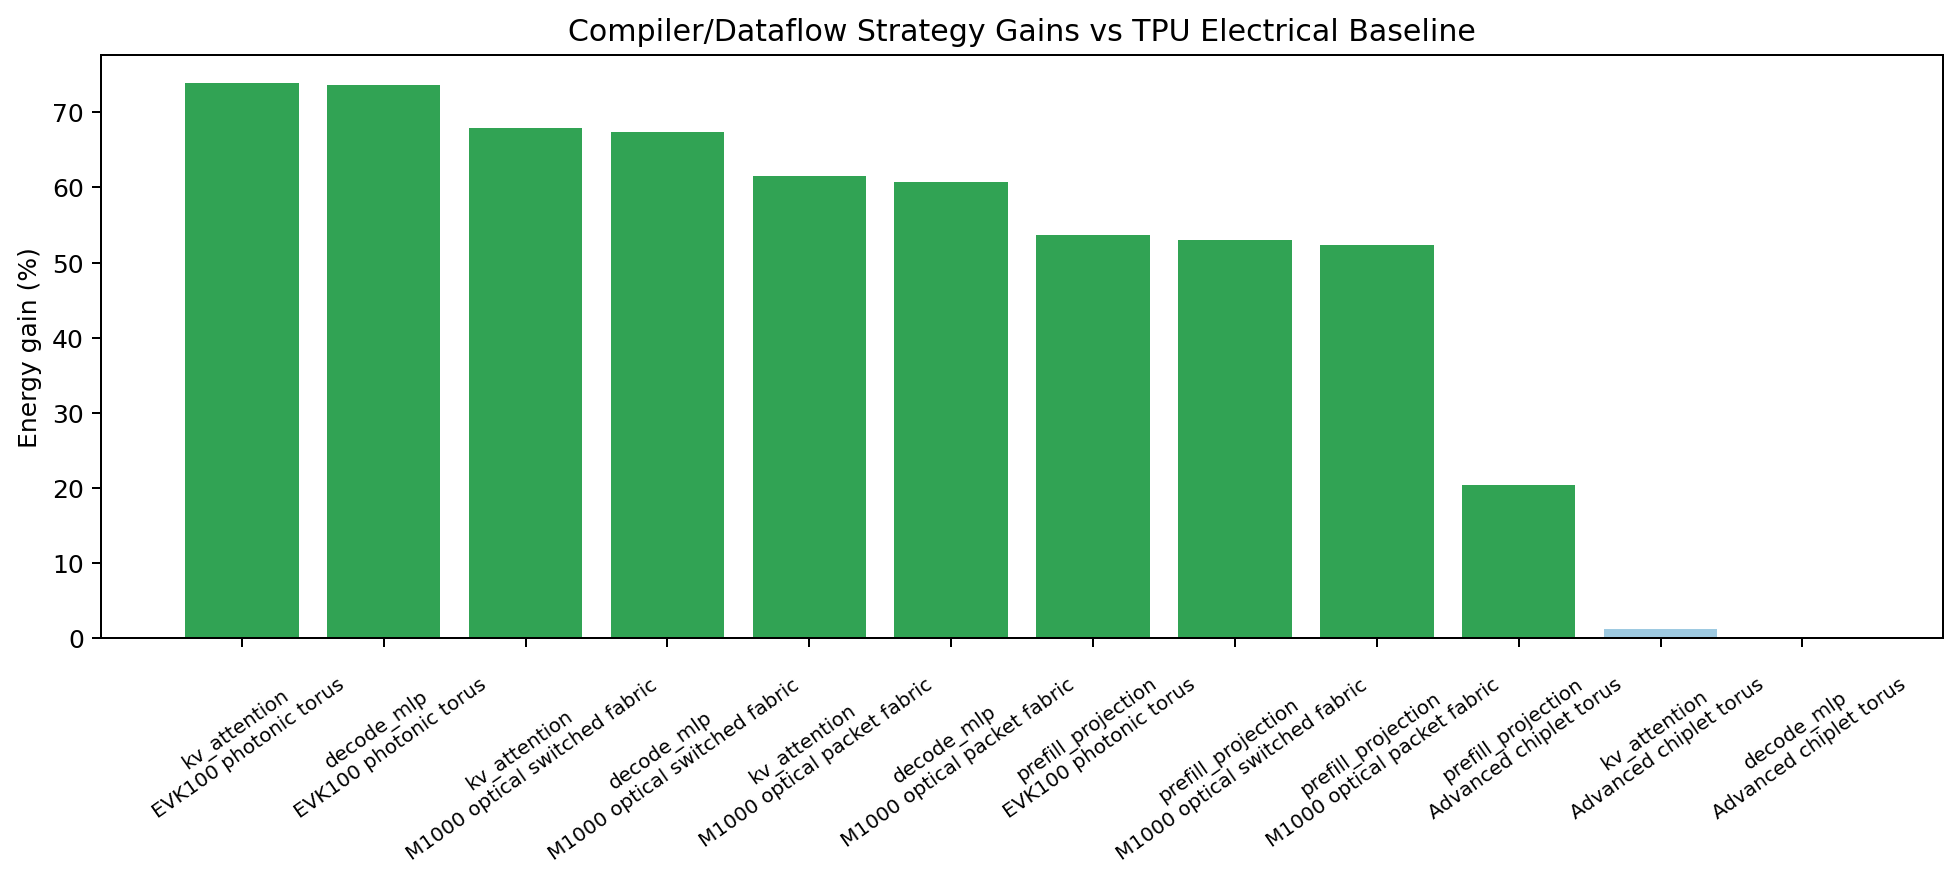
\includegraphics[width=0.97\linewidth]{04_compiler_strategy_choices.png}
\caption{Energy gain of the best distributed schedule per
workload and technology relative to the electrical baseline.
Green bars indicate cases where the optimal compiler-visible
policy switches under photonics.}
\label{fig:compiler}
\end{figure}

\subsection{Pod-scale scaling: where photonics keeps paying}
\label{sec:r-scaling}

The asymmetry above carries through to system scale.
\figref{fig:scaling} reports per-chip shared-state broadcast
latency from cube to pod size on a log--log axis. The TPU
electrical torus and the strong chiplet torus both rise nearly
two orders of magnitude per decade of chip count because they
accumulate hop, contention, and per-mm transmission cost. The
EVK100 photonic torus rises slowly (it inherits hop count even at
near-zero per-mm cost), and the M1000 switched fabric is flat
because it has neither growing hop count nor growing per-mm cost.

\figref{fig:strongweak} reports per-modelled-work-unit latency
for the Gemma~4 26B sparse-MoE proxy under strong scaling (fixed
problem on more chips) and weak scaling (per-chip work held
constant, problem grows with chip count). The full photonic stack
keeps a clear per-work-unit advantage at every modelled chip
count; weak scaling exposes the per-chip cost growth on the
electrical baseline.

\begin{figure}[t]
\centering
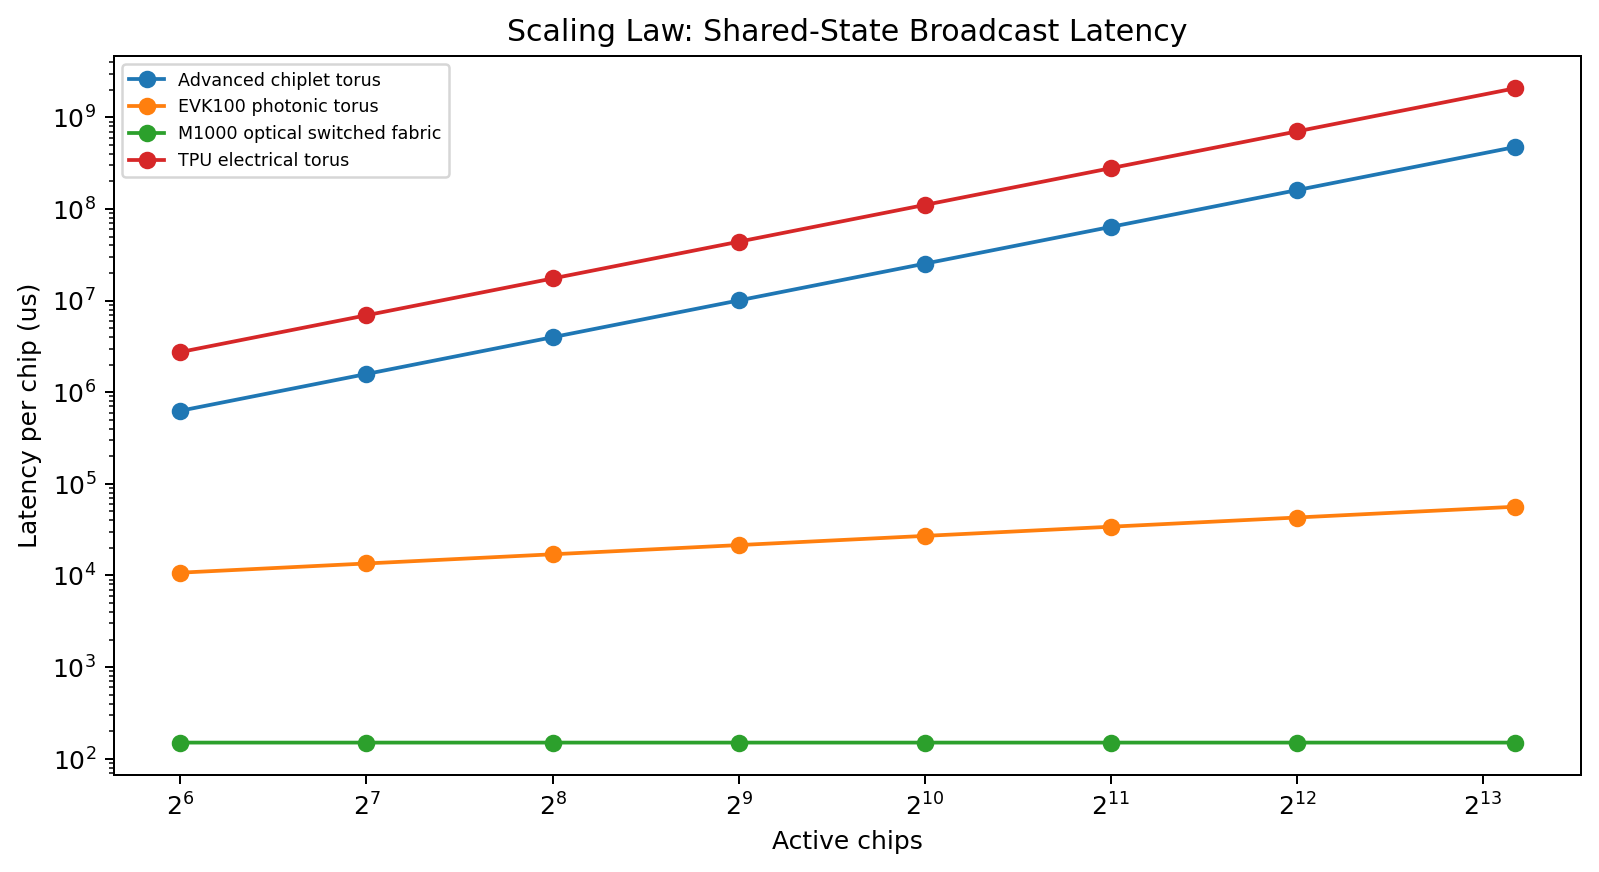
\includegraphics[width=0.97\linewidth]{05_scaling_laws.png}
\caption{Per-chip shared-state broadcast latency from cube to pod
scale. The M1000 switched fabric stays flat across roughly seven
orders of magnitude of separation from the electrical torus at
9216 chips.}
\label{fig:scaling}
\end{figure}

\begin{figure}[t]
\centering
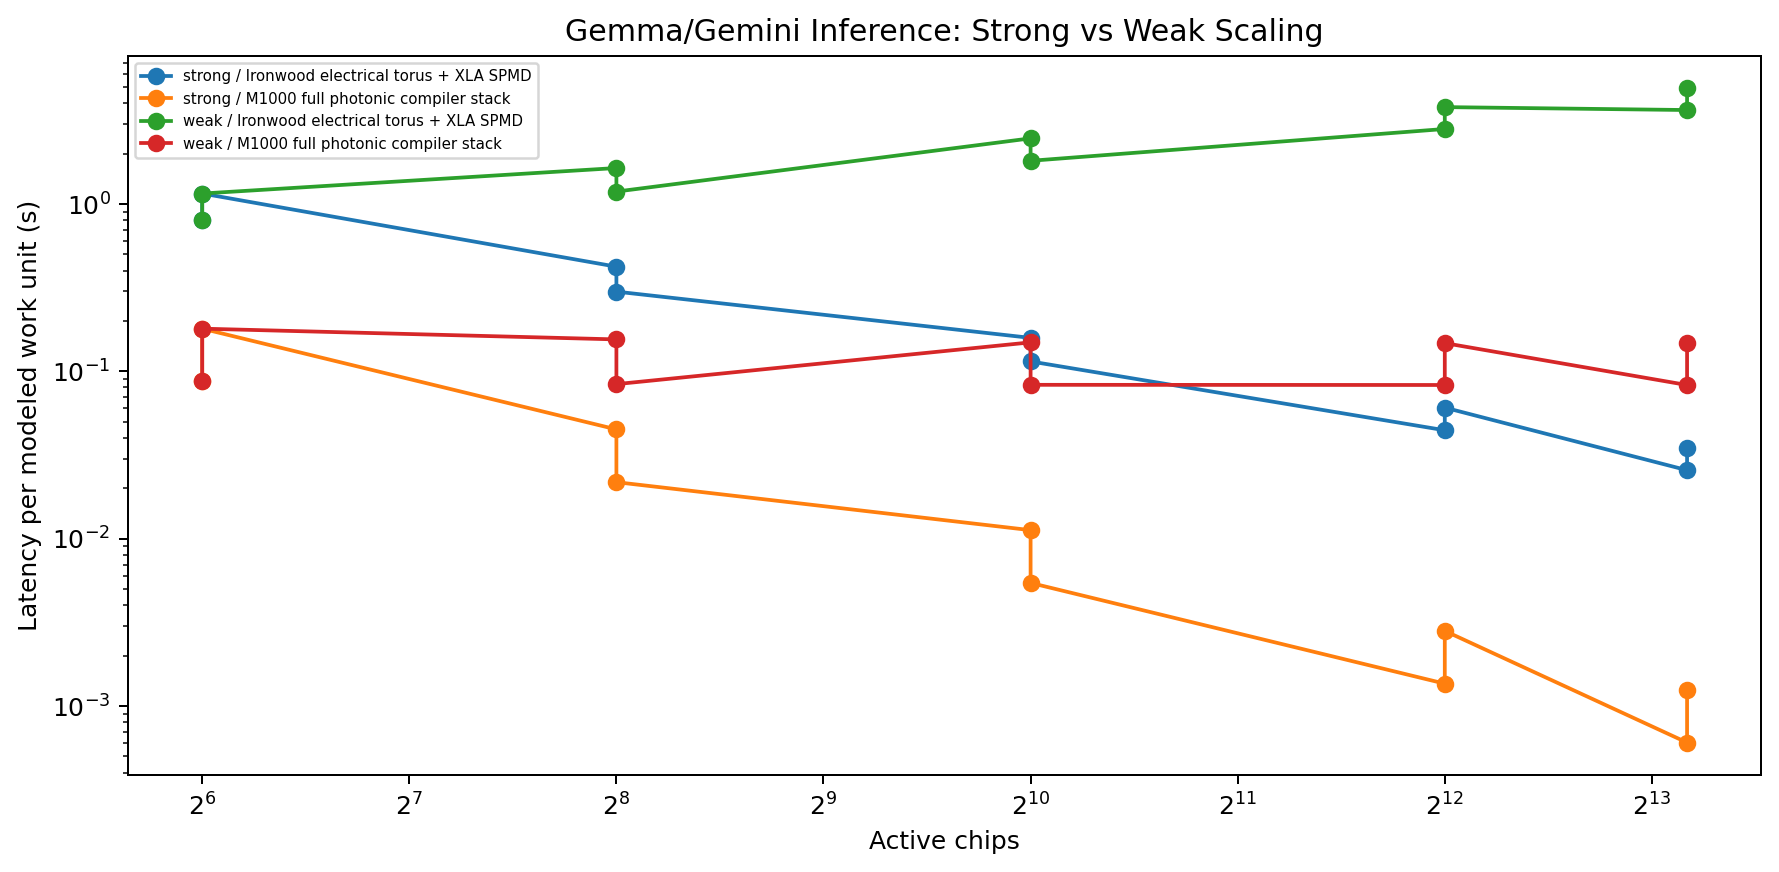
\includegraphics[width=0.97\linewidth]{11_strong_weak_scaling.png}
\caption{Strong and weak scaling on the Gemma~4 26B sparse-MoE
inference proxy. The full photonic stack maintains a clear
advantage; weak scaling exposes the per-chip cost growth on the
electrical baseline.}
\label{fig:strongweak}
\end{figure}

\subsection{End-to-end superpod: inference vs.\ training}
\label{sec:r-superpod}

\figref{fig:superpod} compounds the previous steps onto the
9216-chip Ironwood pod. The Gemma~4 26B sparse-MoE inference
proxy reaches 42.43$\times$ latency speedup and 94.05\% energy
reduction under the full M1000 photonic stack; the larger
long-context Deep Think proxy reaches 14.50$\times$. Training
reaches only 3.37$\times$ on Gemma~4 26B MoE and 1.43$\times$ on
the larger stress proxy.

The reason is visible in the stage decomposition of
\figref{fig:stages}, which plots the per-stage latency that
\emph{remains} once the full photonic stack has been applied. All
inference stages collapse to near zero. The single stage that
does not is training forward/backward compute, which has nothing
to do with the network at all---it sits inside the
$\max(T_c, T_{\text{HBM}})$ envelope. Inference is autoregressive,
so every decoded token continues to pay for KV attention, expert
refill, and a multicast cache fill if available. Training, by
contrast, runs forward, backward, and optimizer steps in tightly
overlapped batches, and once collective and expert traffic are
removed the critical path collapses onto the compute and HBM
envelope that photonics cannot move. The strong case for
photonic interconnect is therefore inference, long-context
serving, and MoE-heavy phases.

\begin{figure}[t]
\centering
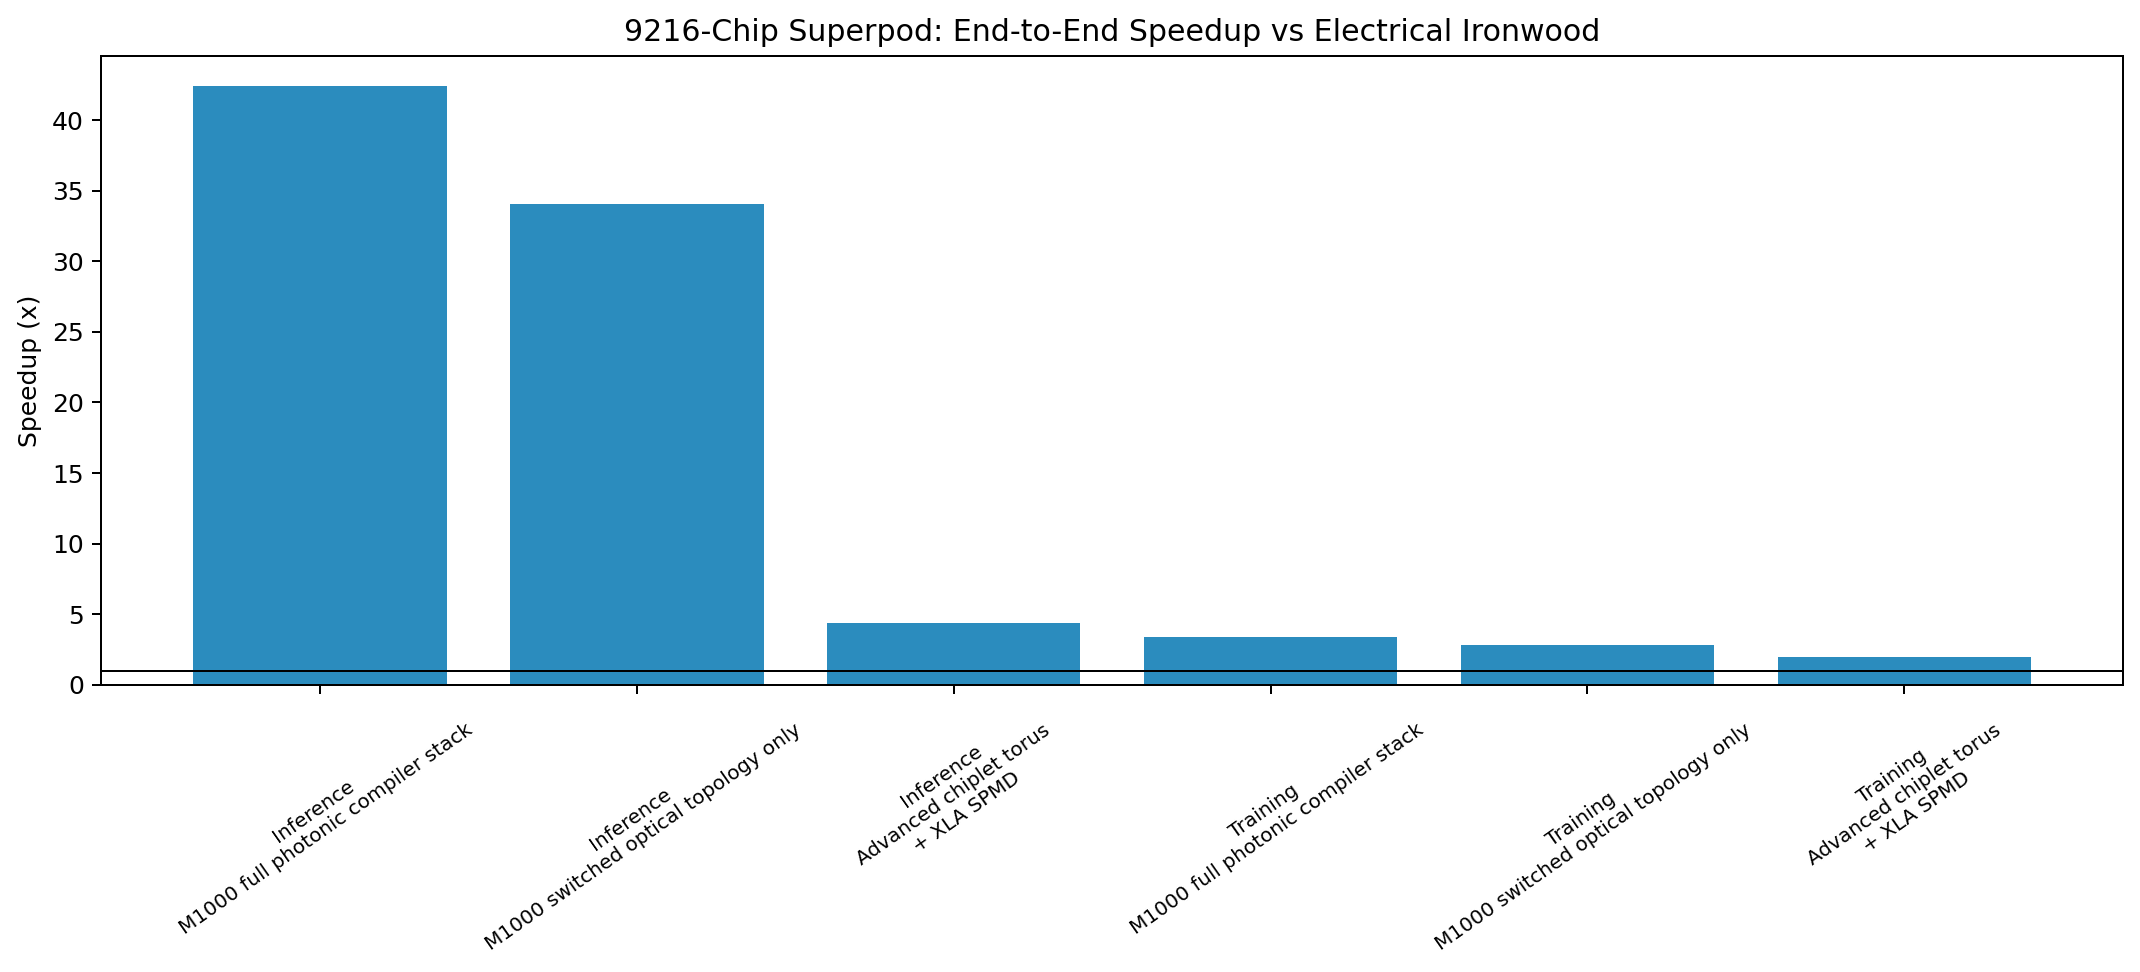
\includegraphics[width=0.97\linewidth]{07_superpod_end_to_end_speedups.png}
\caption{End-to-end speedup on the 9216-chip Ironwood pod.
Inference benefits dramatically more than training under all
photonic configurations.}
\label{fig:superpod}
\end{figure}

\begin{figure}[t]
\centering
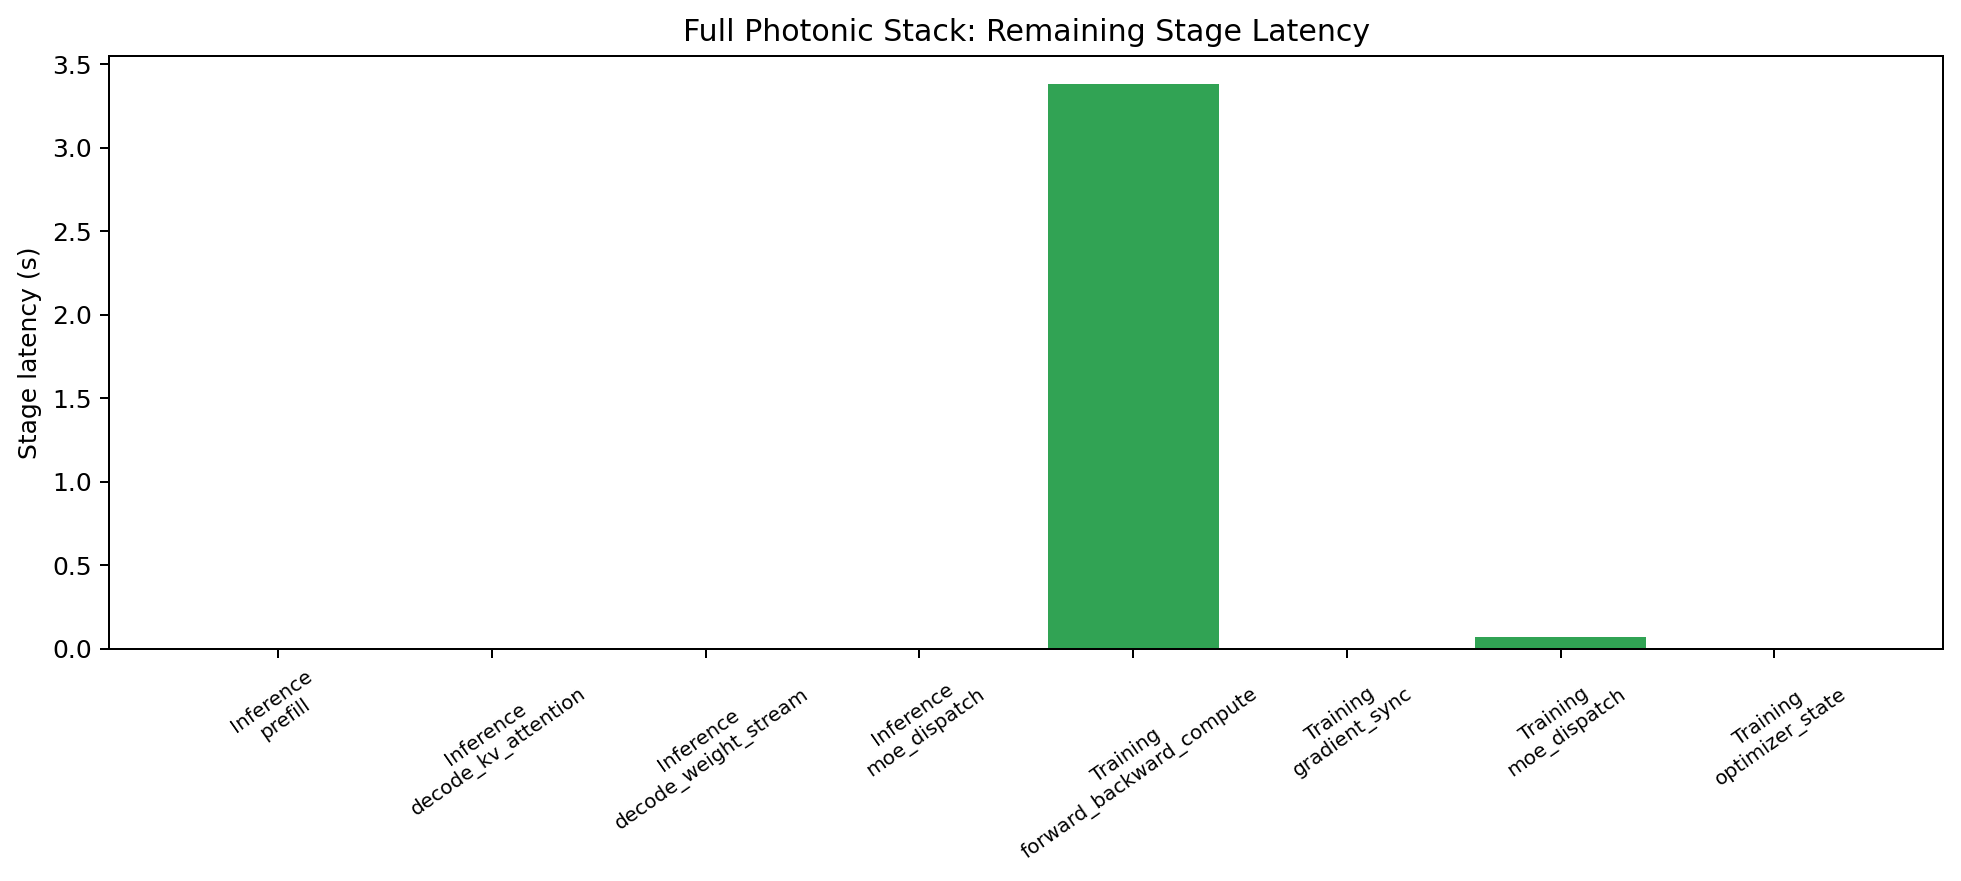
\includegraphics[width=0.97\linewidth]{08_superpod_stage_breakdown.png}
\caption{Per-stage latency that remains under the full M1000
photonic stack. Inference stages collapse to near zero; only
training compute remains, because it is bounded by
$\max(T_c, T_{\text{HBM}})$, not the network.}
\label{fig:stages}
\end{figure}

\subsection{Where it helps, where it does not, and what failed}

Photonics helps most when the workload either fans out to many
chips or repeatedly crosses a long path: long-context inference,
sparse-MoE serving, remote pooled-HBM access, and weight or KV
broadcast. It helps least when the bottleneck is local compute
or per-chip HBM, when the workload is already well served by a
single nearest-neighbour electrical hop, or when the per-chip
mapping was already optimal under the electrical baseline.

The iterative feedback loop and the topology cost model both
behaved as predicted: convergence in three iterations or fewer,
and the multicast asymmetry showed up exactly where physics says
it should. The stage model reproduced the inference--training
divergence cleanly. Two parts of the original plan did not work
as initially designed. Folding the inter-chip network into the
accelerator architecture as a degenerate memory level produced
opaque numbers; the network model is therefore kept external,
with explicit feedback into a single logical-memory level. The
per-chip mapping does not change under any photonic technology;
this is a meaningful negative result and is the empirical
justification for separating the per-chip mapping from the
cluster-level schedule when reporting any new-technology study.

Future work has three natural directions: a direct integration
with an XLA-style compiler so the schedule choice is searched
continuously rather than enumerated; a cycle-accurate simulator
for optical-switch reconfiguration that would tighten the latency
analysis; and a co-design of MoE expert placement under photonic
locality, where the schedule can move the experts as well as the
broadcast.

\section{LLM Usage}
A coding assistant was used during the implementation phase to
write Python plumbing for artifact export, LaTeX formatting, and
notebook scaffolding, and to spot inconsistencies between
deliverables. Architecture decisions, the four-layer modelling
stack, the choice of distributed-schedule families, the
distance-parametrised energy model, the iterative feedback loop,
the analytical stage model, and every numerical interpretation
were authored by the team. The assistant was most helpful for
boilerplate and typesetting and least helpful for design
judgment about what the model should and should not include and
for resolving methodology objections, both of which required
reading the course material directly. Public technology values
were cross-checked against the cited primary sources, and every
result in the paper is reproduced by a single command and a
regression suite that locks in the central physics and the
inference--training asymmetry.

\begin{thebibliography}{99}
\footnotesize

\bibitem{lec03-memory} V. Sze and J. Emer, ``Memory, Metrics,
Einsums, and Transformers,'' MIT 6.5930 lecture notes,
Spring 2026.

\bibitem{lec05-mapping} V. Sze and J. Emer, ``Mapping,''
MIT 6.5930 lecture notes, Spring 2026.

\bibitem{lec06-partitioning} V. Sze and J. Emer, ``Mapping and
Partitioning,'' MIT 6.5930 lecture notes, Spring 2026.

\bibitem{lec11-advtech} V. Sze and J. Emer, ``Advanced
Technologies,'' MIT 6.5930 lecture notes, Spring 2026.

\bibitem{tcm} M. Gilbert, T. Andrulis, V. Sze, and J. S. Emer,
``Turbo-Charged Mapper: Optimal Hardware-Aware Schedules for
DNN Accelerators,'' MIT, 2025.

\bibitem{ciml-photonics} T. Andrulis, G. I. Chaudhry, V. M.
Suriyakumar, J. S. Emer, and V. Sze, ``Architecture-Level
Modeling of Photonic Deep Neural Network Accelerators,''
\emph{ISPASS}, 2024.

\bibitem{lightmatter-passage} Lightmatter, ``Passage product
family,'' viewed Apr.\ 2026.
\url{https://lightmatter.co/products/passage/}

\bibitem{lightmatter-evk100} Lightmatter, ``Passage EVK100,''
viewed Apr.\ 2026.
\url{https://lightmatter.co/products/passage/evk100/}

\bibitem{lightmatter-m1000} Lightmatter, ``Passage M1000 EVK,''
viewed Apr.\ 2026.
\url{https://lightmatter.co/products/passage-m1000-evk/}

\bibitem{lightmatter-l200} Lightmatter, ``Passage L200,''
viewed Apr.\ 2026.
\url{https://lightmatter.co/products/l200/}

\bibitem{lightmatter-tco} R. Jain, ``Scaling AI Infrastructure
with Photonic Interconnects,'' ISES Korea, Aug.\ 2025.
\url{https://lightmatter.co/wp-content/uploads/2025/08/ISES-Korea-08-2025_Ritesh-Jain.pdf}

\bibitem{lightmatter-ocp} Lightmatter, ``OCP CPO reference
architecture initiative,'' Mar.\ 2026.
\url{https://lightmatter.co/press-release/lightmatter-announces-reference-architecture-initiative-with-industry-leaders-in-the-open-compute-project-for-co-packaged-optics/}

\bibitem{tpuv5p} Google Cloud, ``Cloud TPU v5p,'' viewed
Apr.\ 2026. \url{https://cloud.google.com/tpu/docs/v5p}

\bibitem{tpu7x} Google Cloud, ``Cloud TPU7x,'' last updated
Apr.\ 15, 2026.
\url{https://docs.cloud.google.com/tpu/docs/tpu7x}

\bibitem{ironwood-blog} Google Cloud, ``Inside the Ironwood TPU
co-designed AI stack,'' Apr.\ 2026.
\url{https://cloud.google.com/blog/products/compute/inside-the-ironwood-tpu-codesigned-ai-stack/}

\bibitem{hotchips-ironwood} P. Kanwar, ``TPU Rack Scale
Systems,'' Hot Chips 2025 Tutorial, Aug.\ 2025.
\url{https://hc2025.hotchips.org/assets/program/tutorials/HC2025.T1DCRacks.S7.Pankaj.pdf}

\bibitem{xla-spmd} PyTorch/XLA, ``SPMD user guide,'' viewed
Apr.\ 2026.
\url{https://docs.pytorch.org/xla/master/spmd.html}

\bibitem{gemma4-blog} Google, ``Gemma 4 open-model release,''
2026. \url{https://blog.google/technology/developers/gemma-4/}

\end{thebibliography}

\end{document}
